%Vytvoril: Maroš Orsak
%xorsak02
%2017

\documentclass{beamer}
\mode<presentation> {
\usetheme{Warsaw}
\setbeamercovered{transparent}
}
\usecolortheme{whale}

\usepackage[export]{adjustbox} % pouzitie kvoli picture position
\usepackage[utf8]{inputenc}
\usepackage[czech]{babel}
\usepackage{times}
\usepackage{graphics}
\usepackage{amsmath, amsthm, amssymb}

\title{Konečné automaty}
\author{\texorpdfstring{Maroš Orsák \ \newline\url{xorsak02@stud.fit.vutbr.cz}}{Author}}
\institute{Vysoké učenie technické v~Brně \\Fakulta informačných technológií}
\date{25. 4. 2018}

\addto\captionsczech{\renewcommand{\figurename}{Obrázok}}

\begin{document}
\begin{frame}
\titlepage
\end{frame}


%2.strana
\begin{frame}
\frametitle{Popis}
\begin{itemize}
\item (anglicky finite state machine nebo finite automaton) 
\item  výpočetní model primitivního počítače
\item  skládá se z několika stavů a z několika přechodů a který dokáže přijmout nebo zamítnout předané 
slovo.
\item{Zakladné rozdelenie:}
\begin{itemize}
\item{Konečný automat (KA)}
\item{Deterministický konečný automat (DKA)}
\item{Nedeterministický konečný automat (NKA)}
\end{itemize}
\end{itemize}
\end{frame}

% 3.strana
\begin{frame}
\frametitle{Definice}
\begin{itemize}
\item Konečný automat (KA) je pětice: M = ($Q$, $\Sigma$, $R$, $s$, $F$), kde 
\begin{itemize}

\item $Q$ \textit{je konečná množina} vnítřních (řídicích) stavů,
\item{$\Sigma$ je \textit{vstupní abeceda}}
\item $R$ je \textit{konečná množina pravidel tvaru: $pa \rightarrow q$, kde $p$, $q \in Q$, $a \in \Sigma \cup \{\varepsilon\} $}
\item $s \in Q$ je \textit{počáteční stav}
\item $F \subseteq Q$ je množina \textit{koncových stavů}
\end{itemize}



\end{itemize}
\end{frame}
%4%%%%%%%%%%%%%%%%%%%%%%%%
\begin{frame}
\frametitle{Deterministický konečný automat}

\textbf{Konfigurácia DKA}
\begin{itemize}
\item{je dvojica $(q,w) \in K \times \Sigma^*$, kde $q$ je aktuálny stav automatu a $w$ je dosiaľ neprečítaná časť vstupného slova. }
\end{itemize}
\textbf{Krok výpočtu DKA}
\begin{itemize}
\item je relácia $\vdash _{A} $ na konfiguráciach DKA definovaná nasledovne:$(q,av)\vdash _{A}(p,v)\iff p=\delta (q,a).$
\item rozumieme ľubovoľnú postupnosť na seba nadväzujúcich výpočtových krokov.
\end{itemize}

\textbf{Jazyk akceptovaný pomocou DKA}
\begin{itemize}
\item definujeme nasledovne:
\begin{itemize}
\item $L(A)=\{w\ |\ \exists p\in F:(q_{0},w)\vdash _{A}^{\ast }(p,\varepsilon )\}.$
\end{itemize}

\item  množina všetkých slov
 na ktorých existuje v automate A výpočet končiaci v akceptačnom stave (takému výpočtu sa tiež hovorí akceptačný výpočet).
\end{itemize}
\end{frame}
%5%%%%%%%%%%%%%%%%%%%%%%%
\begin{frame}
\frametitle{Nedeterministický konečný automat}

\textbf{Konfigurácia NKA}
\begin{itemize}
\item{definuje sa  analogicky, ako pri deterministických konečných automatoch}
\item dvojica $(q,w)\in K\times \Sigma ^{\ast }$, kde q je aktuálny stav automatu a w je dosiaľ neprečítaná časť vstupného slova.
\end{itemize}
\textbf{Krok výpočtu NKA}
\begin{itemize}
\item{je relácia  $\vdash A $ na konfiguráciach NKA A definovaná nasledovne:}
\begin{itemize}
\item $(q,aw)\vdash _{A}(p,w)\iff p\in \delta (p,a).$
\end{itemize}
\end{itemize}
\textbf{Jazyk akceptovaný pomocou NKA}
\begin{itemize}
\item Jazyk akceptovaný nedeterministickým konečným automatom A je množina
\begin{itemize}

\item $L(A)=\{w\ |\ \exists p\in F:(q_{0},w)\vdash _{A}^*(p,\varepsilon )\}.$

\end{itemize}
\end{itemize}


\end{frame}
%6%%%%%%%%%%%%%%%%%%%%%%%%%
\begin{frame}
\frametitle{Ekvivalencia DKA a NKA}
% TOTO SI PREPIS POTOM...
\begin{itemize}
\item{V skutočnosti, napriek rozdielnej definícii oboch výpočtových modelov, je ich výpočtová sila rovnaká
\item Je dokázané, že ku každému nedeterministickému automatu A existuje deterministický konečný automat B taký, že L(B) = L(A)
\item  Opačná inklúzia je zrejmá z faktu, že deterministický automat je špeciálny prípad nedeterministického.}
\end{itemize}
\end{frame}

%NKA 7%%%%%%%%%%%%%%%%%% % ASI sem este dopln jeden obrazok DKA.... 
\begin{frame}
\frametitle{NKA}
\begin{figure}[Htbp]
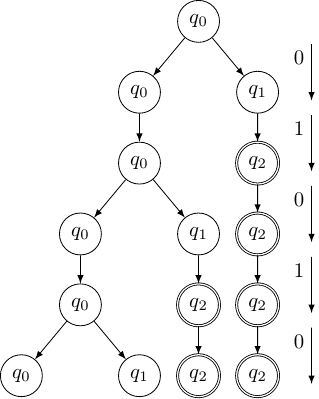
\includegraphics[scale = 0.70]{nedeterministicky-konecny-automat-5fb817ed126c31736b4a776ce42cc7cc.png}
\caption{Nedeterministický konečný automat }
\end{figure}
\end{frame}


%8.strana DKA vs NKA %%%%%%%%%%%%%%%%%%
\begin{frame}
\frametitle{DKA vs NKA}
\begin{figure}[Htbp]
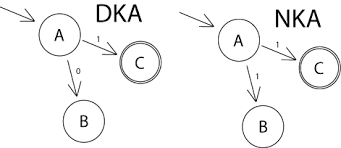
\includegraphics[scale = 0.68]{DKA_vs_NKA.png}
\caption{DKA vs NKA}
\end{figure}
\end{frame}

%9.strana DKA ,NKA %%%%%%%%%%%%%%%%%%
\begin{frame}
\frametitle{DKA , NKA}
\begin{figure}[Htbp]
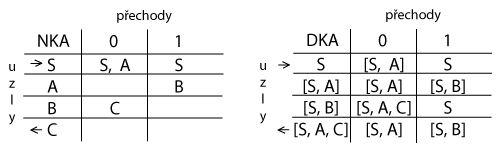
\includegraphics[scale = 0.50]{NKA_DKA.png}
\caption{Prevod nedeterministickáho automatu na deterministický }
\end{figure}
\end{frame}


%10.strana%%%%%%%%%%%%%%%%%%%%%%%%
\begin{frame}
\frametitle{Použitá literatúra}
\begin{itemize}
\item{Alexander Meduna, Roman Lukáš : Formální jazyky a překladače IFJ Studijní opora }
\item{\texttt{https://matematika.cz/konecny-automat}}
\item{\texttt{https://sk.wikipedia.org/wiki/Konečný automat}}


\end{itemize}
\end{frame}

\end{document}


